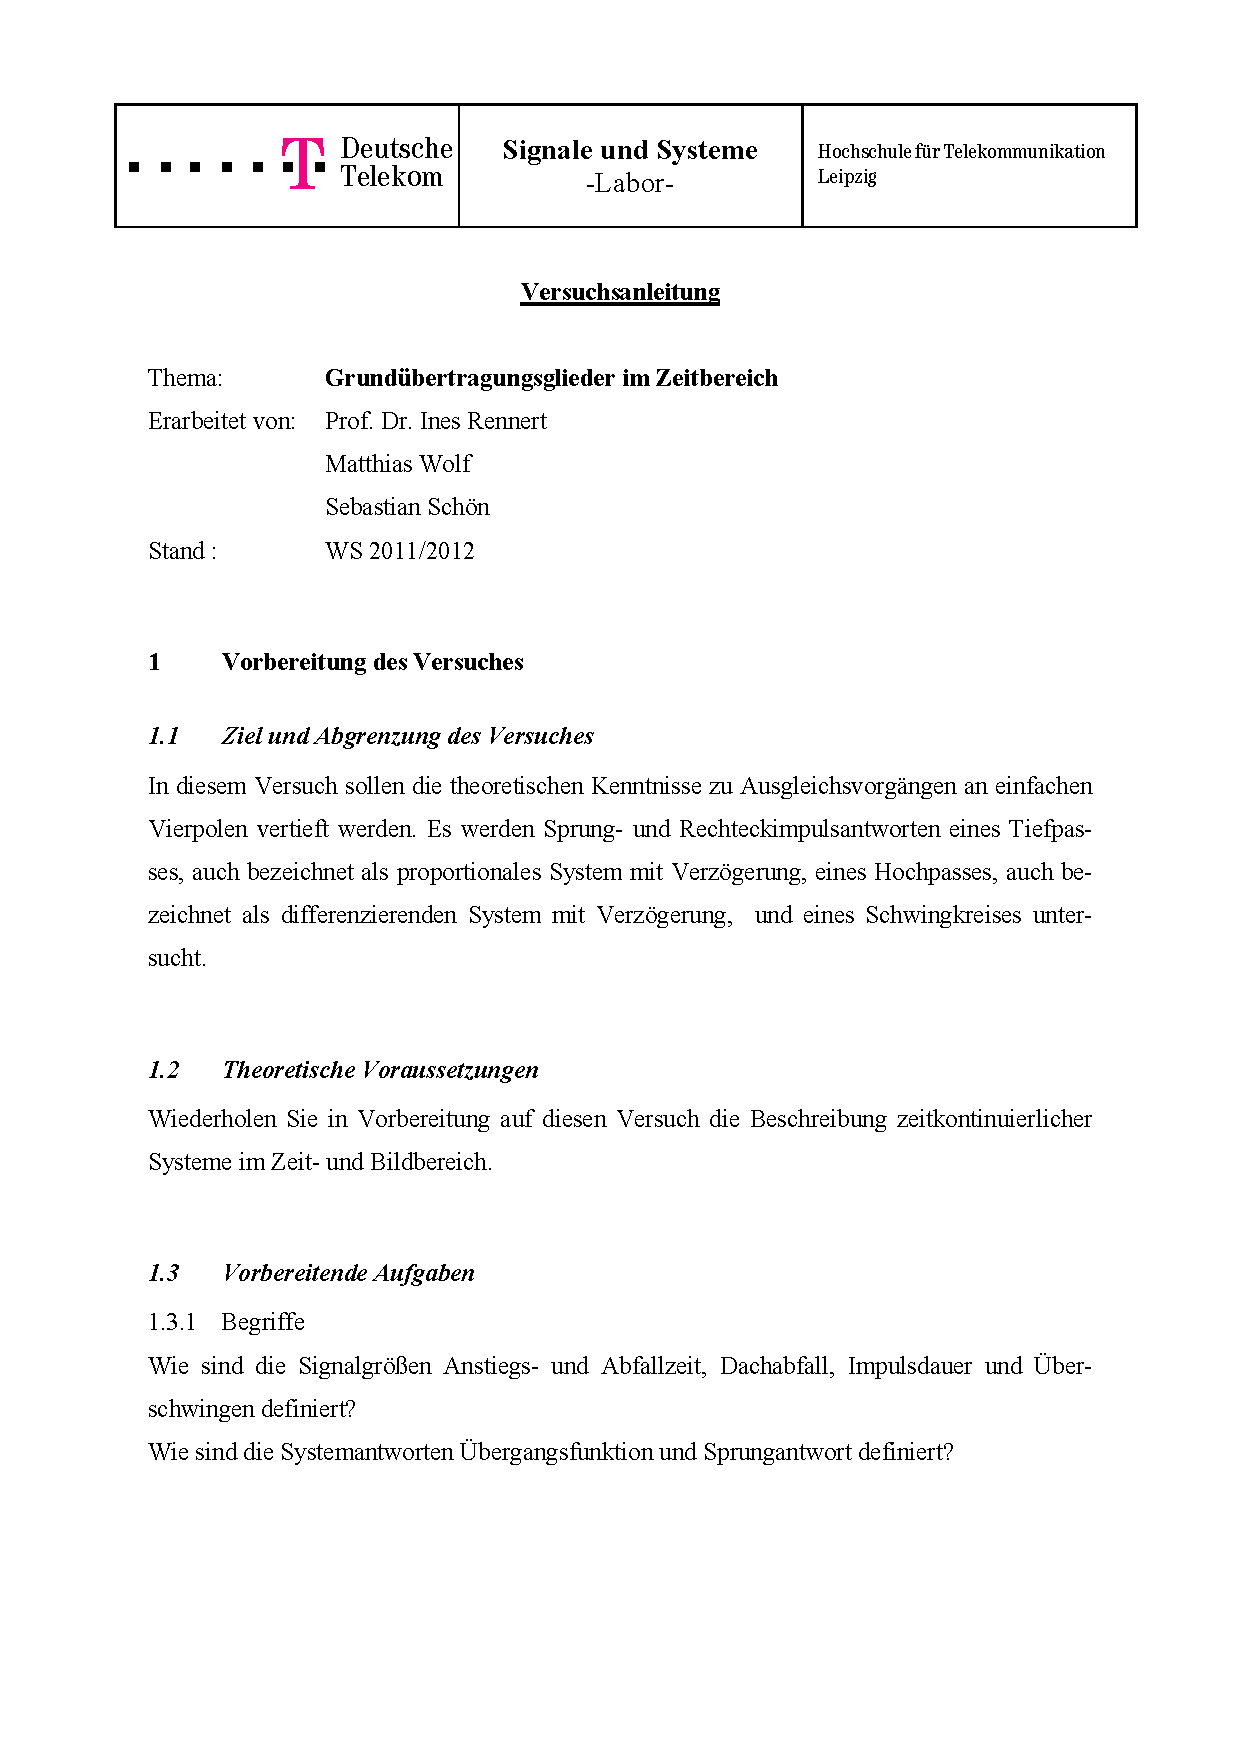
\includegraphics[width=1.0\textwidth]{Bilder/Grundubertragungsglieder im Zeitbereich (verschoben)}\newpage
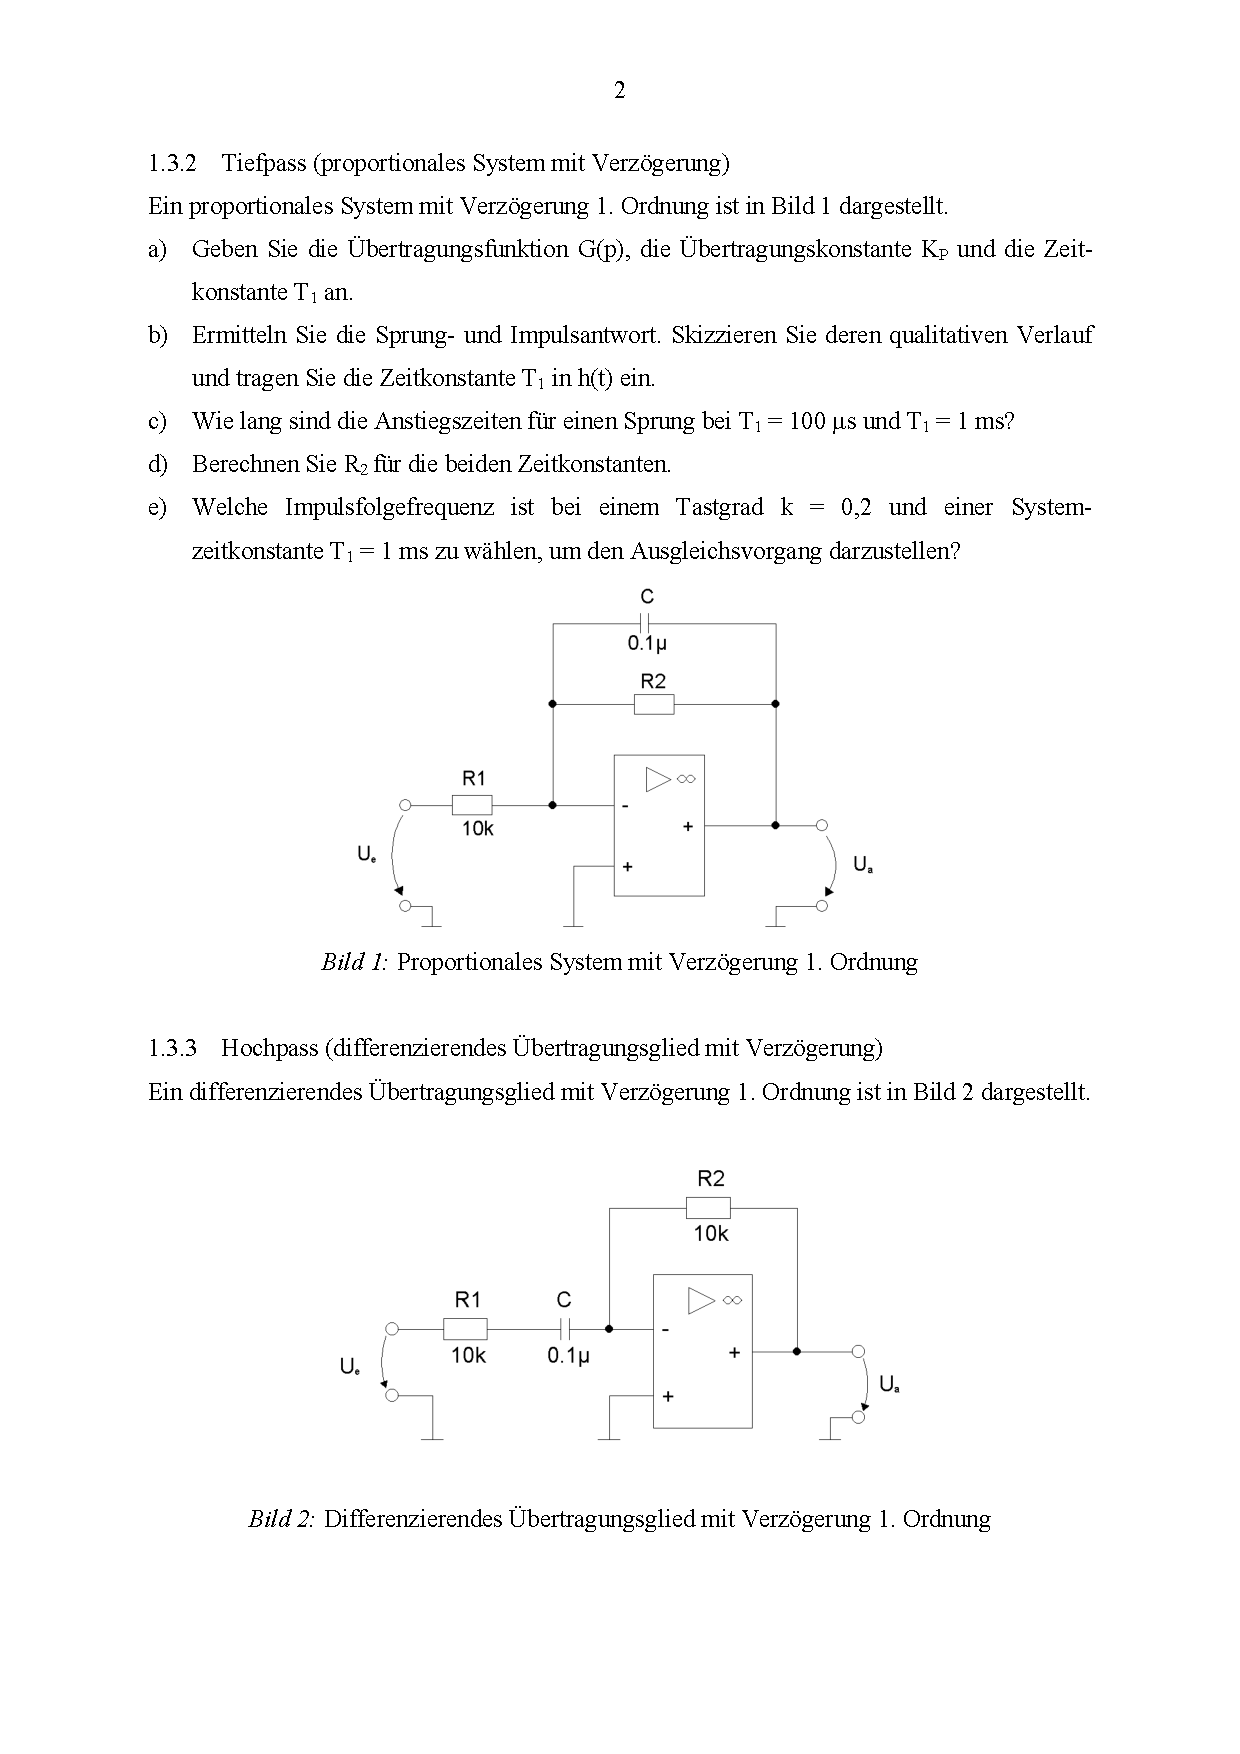
\includegraphics[width=1.0\textwidth]{Bilder/Grundubertragungsglieder im Zeitbereich (verschoben) 2}\newpage
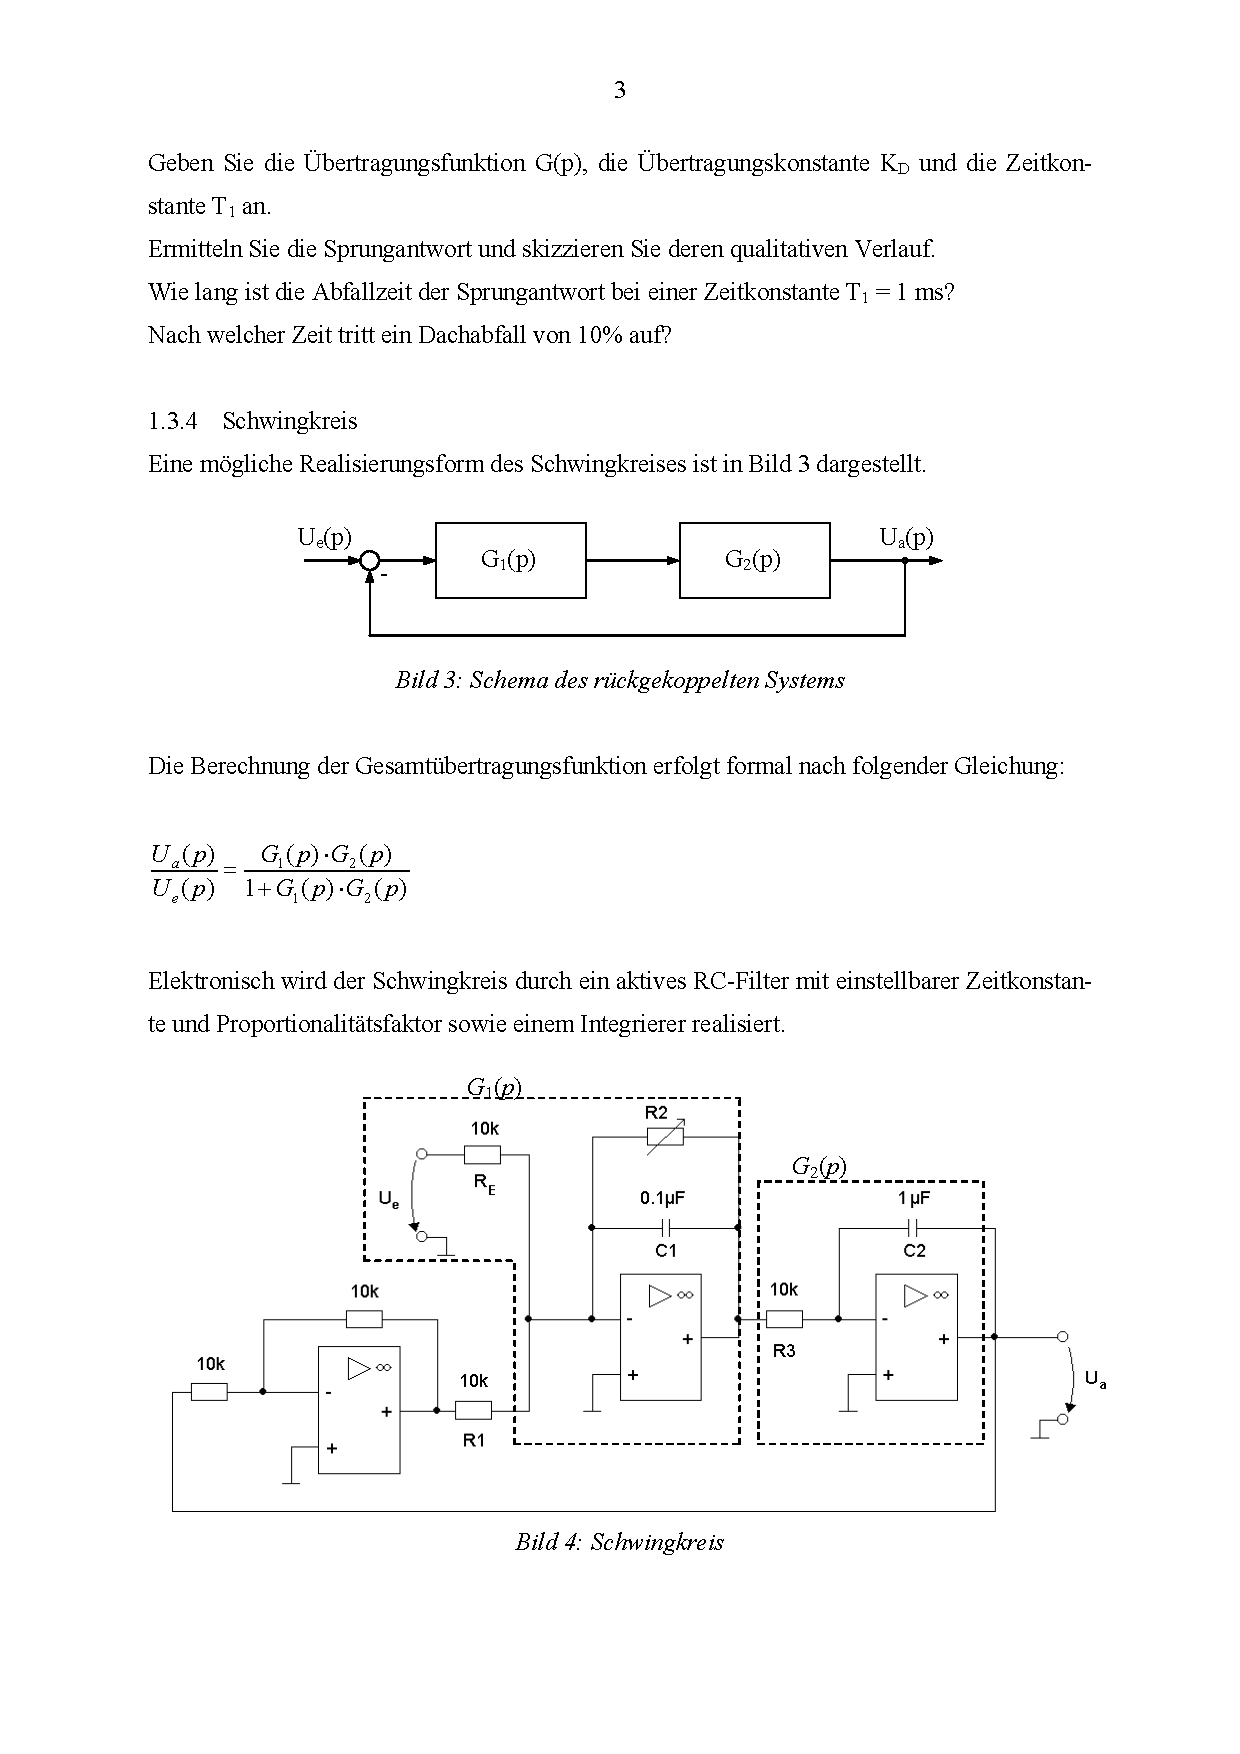
\includegraphics[width=1.0\textwidth]{Bilder/Grundubertragungsglieder im Zeitbereich (verschoben) 3}\newpage
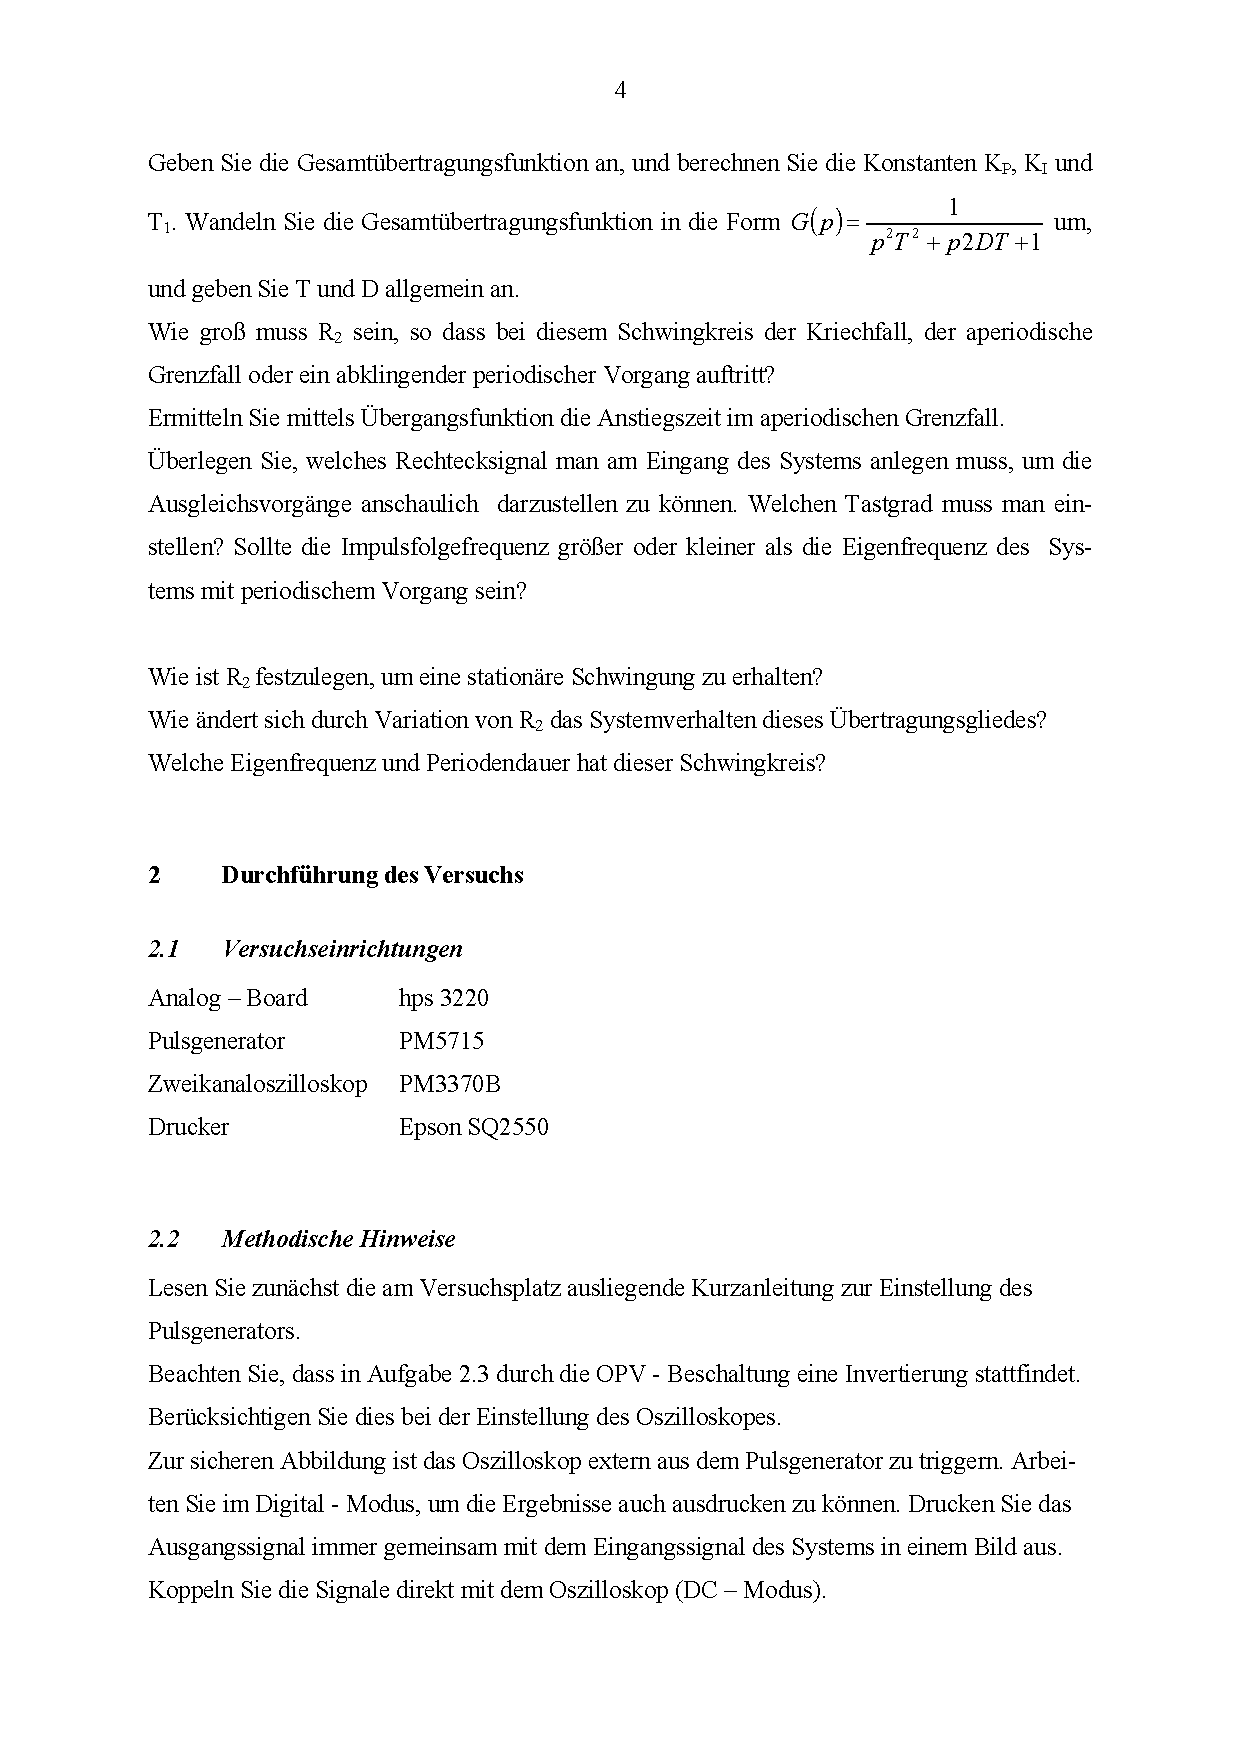
\includegraphics[width=1.0\textwidth]{Bilder/Grundubertragungsglieder im Zeitbereich (verschoben) 4}\newpage
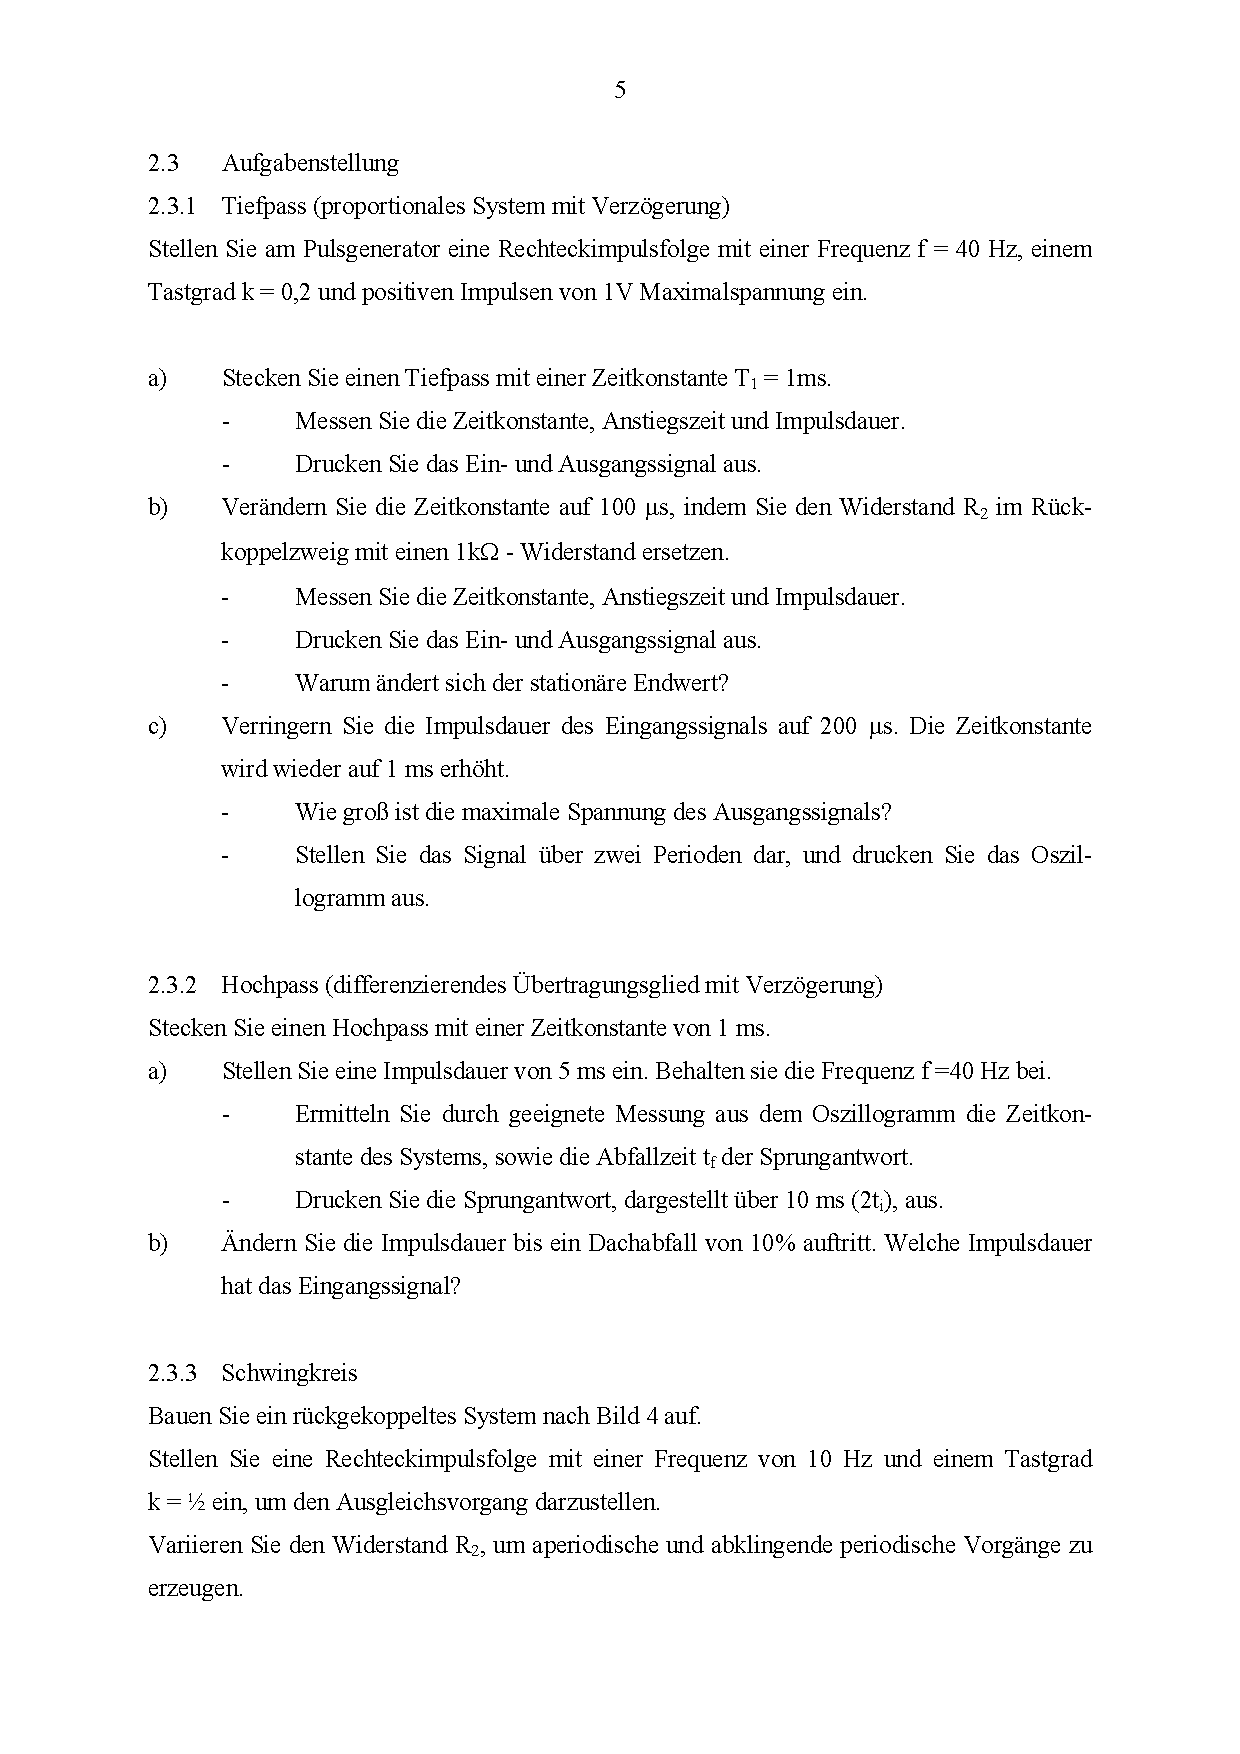
\includegraphics[width=1.0\textwidth]{Bilder/Grundubertragungsglieder im Zeitbereich (verschoben) 5}\newpage
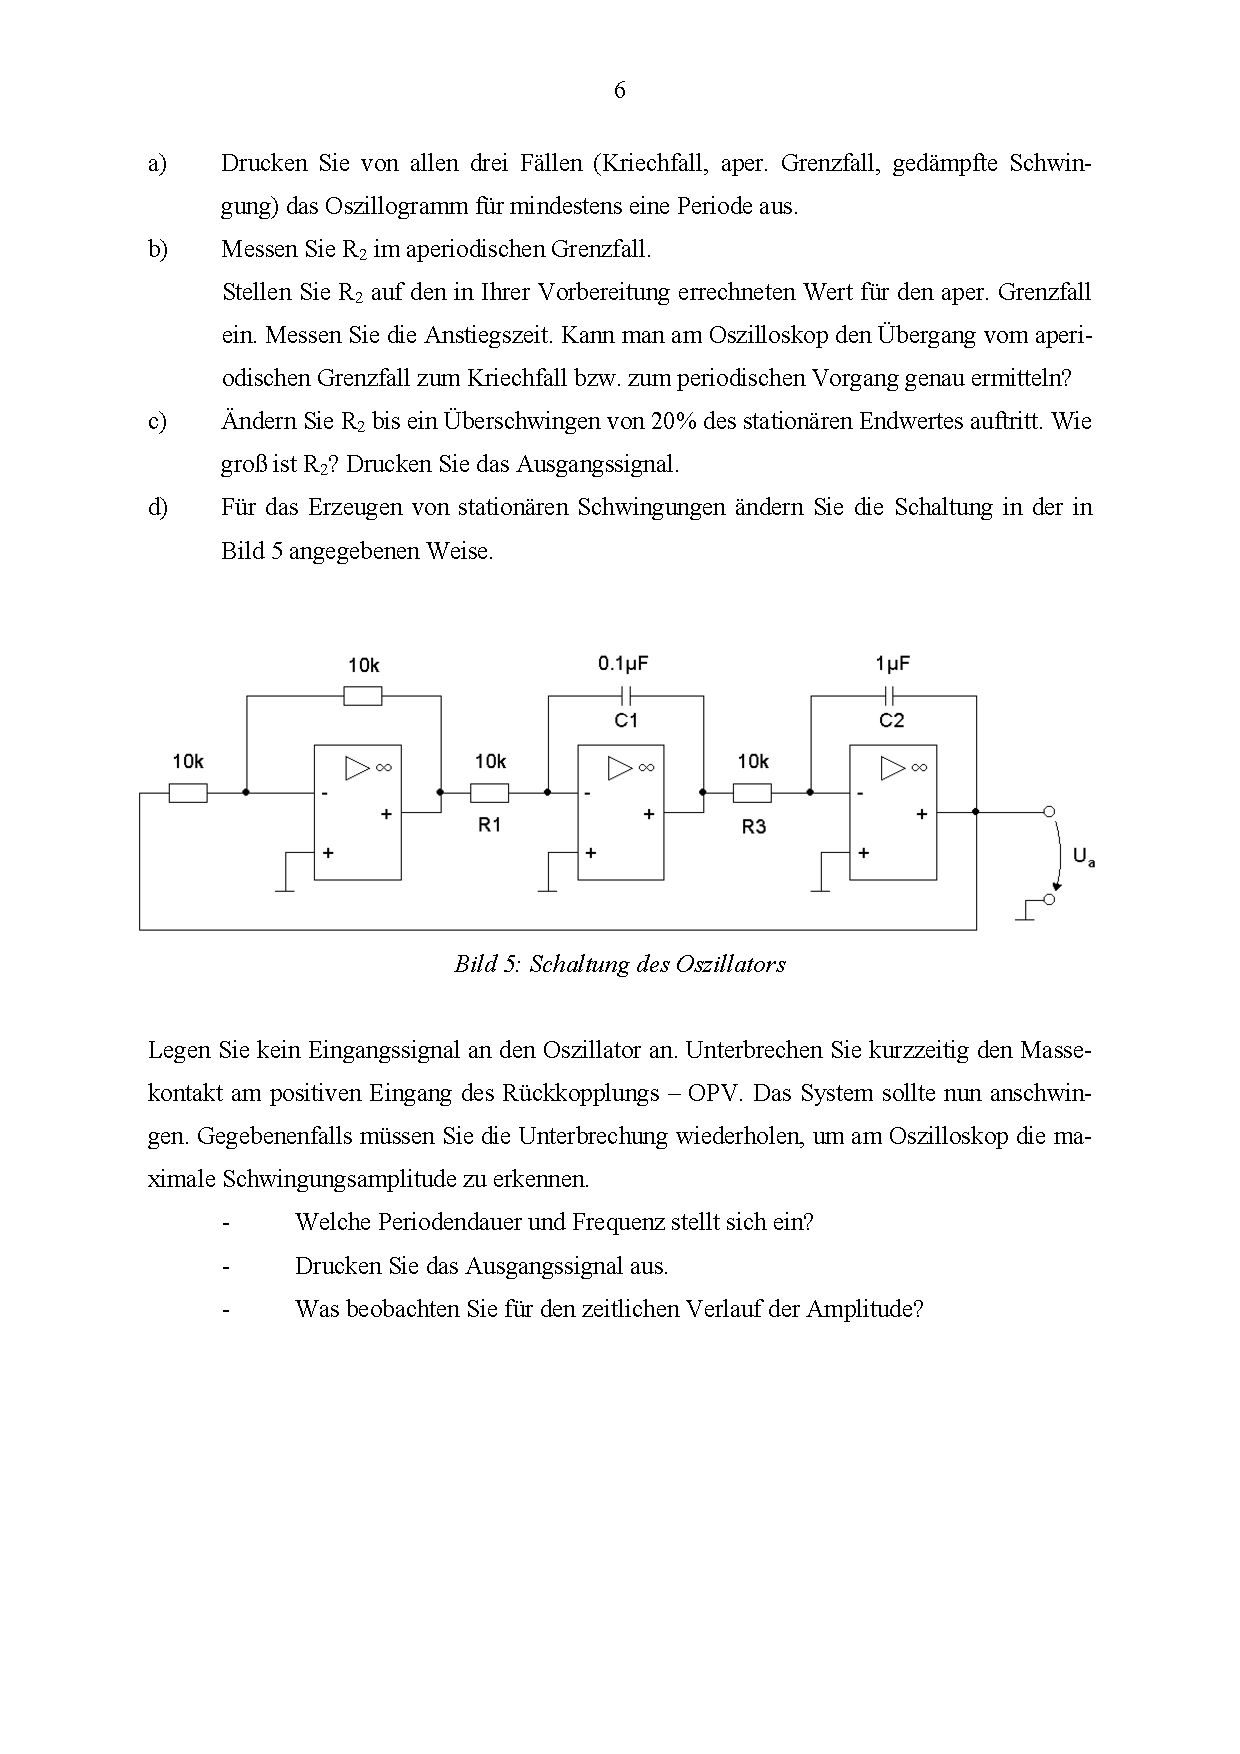
\includegraphics[width=1.0\textwidth]{Bilder/Grundubertragungsglieder im Zeitbereich (verschoben) 6}\newpage
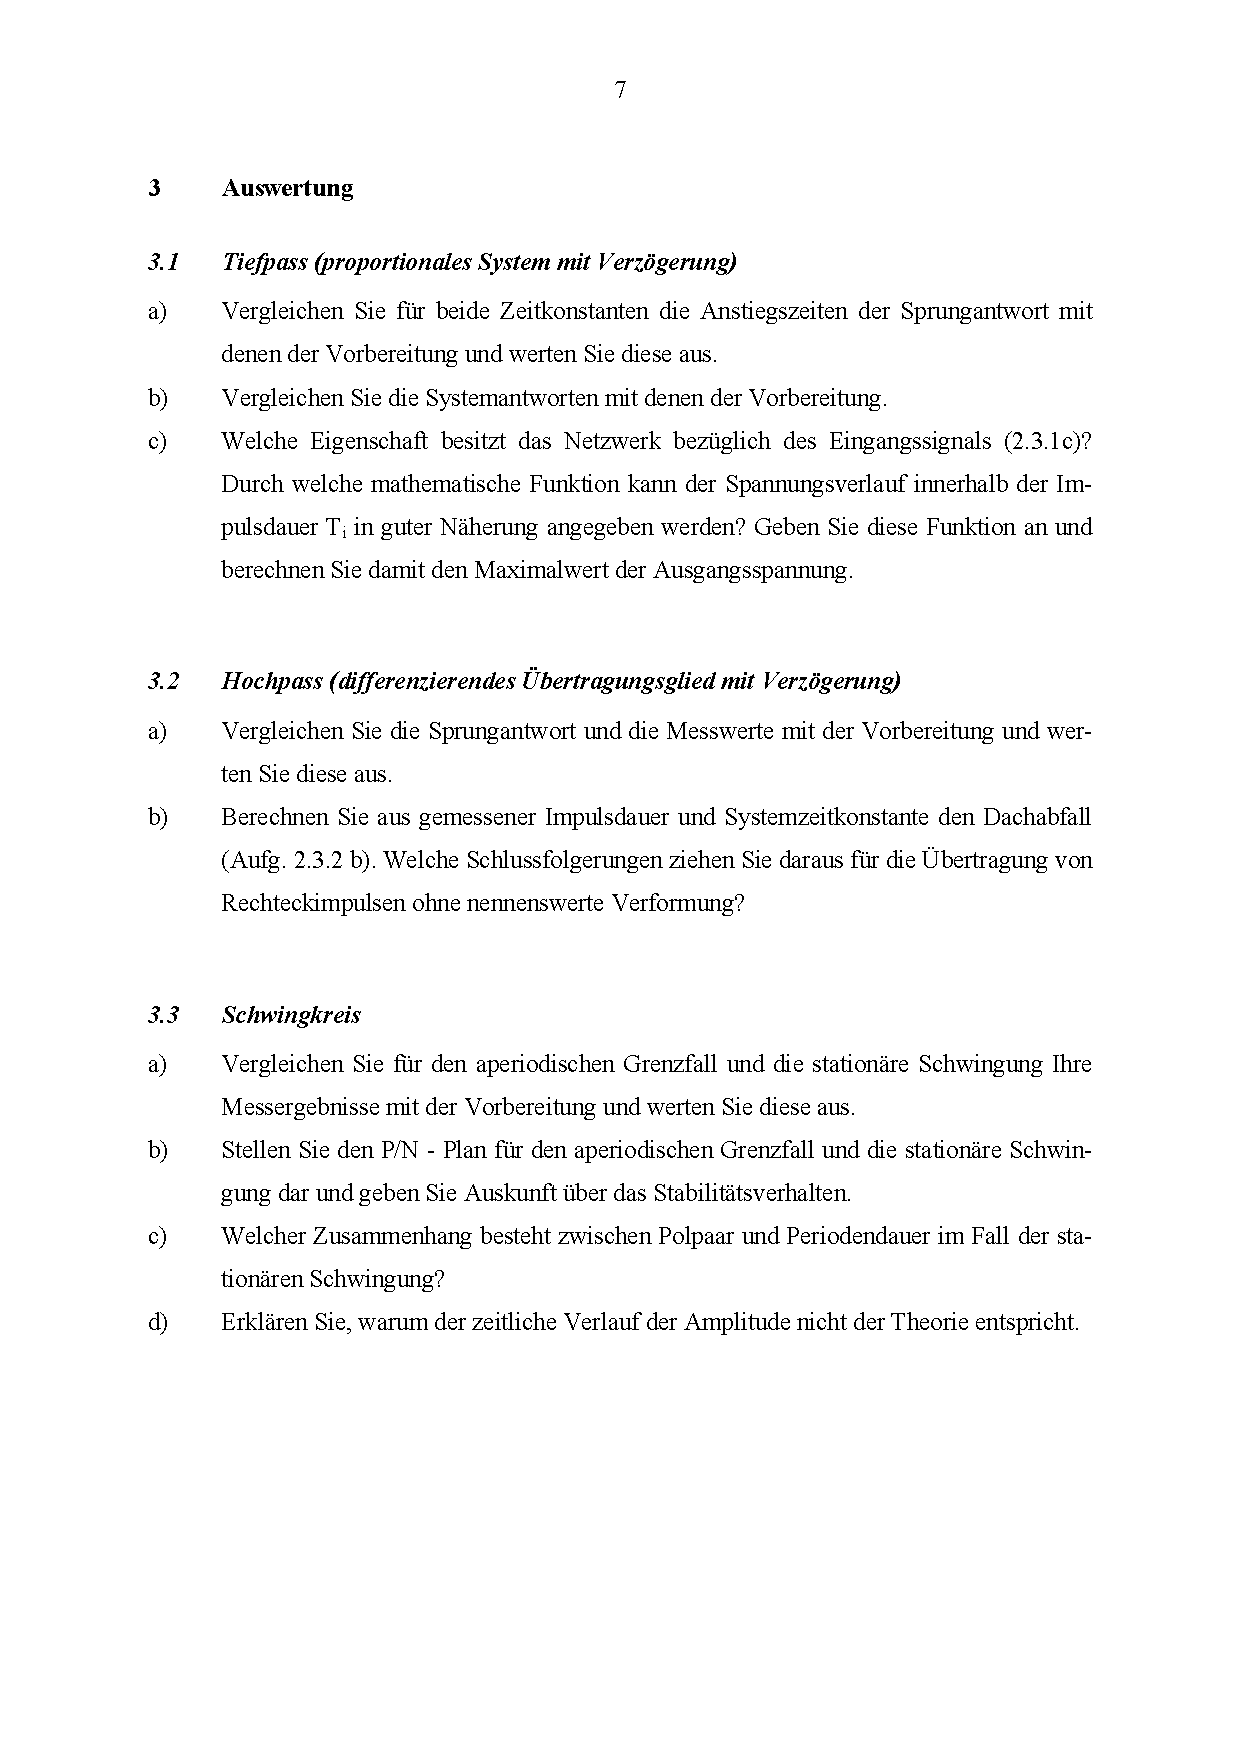
\includegraphics[width=1.0\textwidth]{Bilder/Grundubertragungsglieder im Zeitbereich (verschoben) 7}\newpage


\section{Vorbereitung des Versuches}
\subsection{Ziel und Abgrenzung des Versuches}

In diesem Versuch sollen die theoretischen Kenntnisse zu Ausgleichsvorgängen an 
einfachen Vierpolen vertieft werden. Es werden Sprung- und Rechteckimpulsantworten eines 
Tiefpasses, auch bezeichnet als proportionales System mit Verzögerung,eines Hochpasses, 
auch bezeichnet als differenzierenden System mit Verzögerung, und eines Schwingkreises untersucht.\\
\newline

\subsection{TheoretischeVoraussetzungen}

Wiederholen Sie in Vorbereitung auf diesen Versuch die Beschreibung 
zeitkontinuierlicher Systeme im Zeit- und Bildbereich.
\newline

\subsection{Vorbereitende Aufgaben}
\subsubsection{Begriffe}
Wie sind die Signalgrößen Anstiegs- und Abfallzeit, Dachabfall, Impulsdauer und Überschwingen definiert?\\
%TODO
Wie sind die Systemantworten Übergangsfunktion und Sprungantwort definiert?\\
%TODO
\subsubsection{Tiefpass (proportinales System mit Verzögerung)}
Ein proportionales System mit Verzögerung 1. Ordnung ist in Bild 1 dargestellt.\\
a)    Geben  Sie  die  Übertragungsfunktion  $G(p)$,  die  Übertragungskonstante  KP und die Zeit-konstante T1 an.\\ 
%TODO
b)    Ermitteln  Sie  die  Sprung-  und  Impulsantwort. Skizzieren  Sie  deren  qualitativen  Verlauf und tragen Sie die Zeitkonstante T1 in h(t) ein.\\ 
%TODO
c)    Wie lang sind die Anstiegszeiten für einen Sprung bei $T_{ 1 }=100\mu s$ und $T1 = 1 ms$?\\ 
%TODO
d)    Berechnen Sie R2 für die beiden Zeitkonstanten.\\ 
%TODO
e)    Welche Impulsfolgefrequenz ist bei einem Tastgrad $k = 0,2$ und einer System-zeitkonstante $T1 = 1 ms$ zu wählen, um den Ausgleichsvorgang darzustellen\\
%TODO
\subsubsection{Hochpass (differenzierendes Übertragungsglied mit Verzögerung)}
Ein differenzierendes Übertragungsglied mit Verzögerung 1. Ordnung ist in Bild 2 dargestellt.\\
Geben  Sie  die  Übertragungsfunktion $G(p)$,  die  Übertragungskonstante  KD und die Zeitkon-stante $T1$ an.\\ 
Ermitteln Sie die Sprungantwort und skizzieren Sie deren qualitativen Verlauf.\\ 
Wie lang ist die Abfallzeit der Sprungantwort bei einer Zeitkonstante $T1 = 1 ms$?\\ 
Nach welcher Zeit tritt ein Dachabfall von $10\%$ auf ?\\
\subsubsection{Schwingkreis}
Eine mögliche Realisierungsform des Schwingkreises ist in Bild 3 dargestellt.\\

Die Berechnung der Gesamtübertragungsfunktion erfolgt formal nach folgender Gleichung: \\
\begin{equation}
	\frac{ U_{ a }(p) }{ U_{ e }(p) } =\frac{ G_{ 1 }(p)*G_{ 2 }(p) }{ 1+G_{ 1 }(p)*G_{ 2 }(p)  }
\end{equation}
Elektronisch wird der Schwingkreis durch ein aktives RC-Filter mit einstellbarer Zeitkonstante
und Proportionalitätsfaktor sowie einem Integrierer realisiert.\\
Geben Sie die Gesamtübertragungsfunktion an, und berechnen Sie die Konstanten KP, KI und T1. 
Wandeln Sie die Gesamtübertragungsfunktion in die Form $G(p)=\frac{ 1 }{ p^{ 2 }T^{ 2 }+p2DT+1  }$ um, und geben Sie T und D allgemein an. 
Wie groß muss R2 sein, sodass bei diesem Schwingkreis der Kriechfall, der aperiodische Grenzfall oder ein 
abklingender periodischer Vorgang auftritt?\\
%TODO
Ermitteln Sie mittels Übergangsfunktion die Anstiegszeit im 
aperiodischen Grenzfall. \\
Überlegen Sie, welches Rechtecksignal man am Eingang des Systems anlegen muss, um die 
Ausgleichsvorgänge anschaulich darzustellen zu können. Welchen Tastgrad muss man einstellen?\\
%TODO 
Sollte die Impulsfolgefrequenz größer oder kleiner als die Eigenfrequenz des Systems mit periodischem Vorgang sein?\\
%TODO
Wie ist R2 festzulegen, um eine stationäre Schwingung zu erhalten?\\
%TODO 
Wie ändert sich durch Variation von R2 das Systemverhalten dieses Übertragungsgliedes?\\
%TODO 
Welche Eigenfrequenz und Periodendauer hat dieser Schwingkreis?\\
%TODO

\section{Durchführung des Versuchs}
\subsection{Versuchseinrichtung}
\subsection{Methodische Hinweise}
\subsection{Aufgabenstellung}
\subsubsection{Tiefpass (proportinales System mit Verzögerung)}
\subsubsection{Hochpass (differenzierendes Übertragungsglied mit Verzögerung)}
\subsubsection{Schwingkreis}
\section{Auswertung}
\subsection{Tiefpass (proportinales System mit Verzögerung)}
\subsection{Hochpass (differenzierendes Übertragungsglied mit Verzögerung)}
\subsection{Schwingkreis}

